\subsection{Power Distribution Board - Alexander Falk}
The redesign of the Butler demanded new electronics and motors. This meant that a new Power Distribution Board (PDB) was needed. The PDB is one of the fundamental parts of the Butler since it supplies power to all the electronics and motors in order for the Butler to operate. See the manual on Teams for the comprehensive view of the components and layout\footnote{Butler PDB - butler\_pdb.pdf on Microsoft Teams}.
\subsubsection{Requirements}
The main requirements involve the correct voltage levels and current ratings. From the specifications, see table \ref{table: Power requirements for the Butler}, the voltage levels that is required are 5 V, 12 V and maximum 14 V. The motors together would require about 7 A. The Cortex M4f has an USB connector for the power and that is rated for a maximum of 500 mA at 5 V. The Jetson TX2 power adapter is rated 90 W and at 12 V equals 7.5 A.

Then there was requirements regarding safety. The Butler should be able to be stopped in case of an error. It was desired to have minimum of an emergency switch for the arm and a magnetic switch for the motors that drive the Butler forward.

The last requirement involve the ability to measure the voltage and current in order to see the utilisation and evaluate the performance.
\subsubsection{Overview}
The PDB for the Butler Project is designed to supply power to the motors and additional electronics. The PDB is divided in five separate boards (see figure \ref{fig:butlerpdb}): Power Board, Safety Switch Board, Motor Board, Aux (Auxiliary) Board and Arduino Board. The PDB have safety functions which enables the control electronics to be powered but having the motors disabled. The Power Board also has the ability to measure the voltage and current with a voltage/current monitor. The voltage/current Monitor communicates via I\textsuperscript{2}C bus connected to the Arduino Board. The Arduino Board is designed to have a Arduino Micro mounted and have all outputs available to facilitate different communication needs. All digital signals of the boards operate at 5 V logic levels.

\begin{figure}[ht!]
\centering 
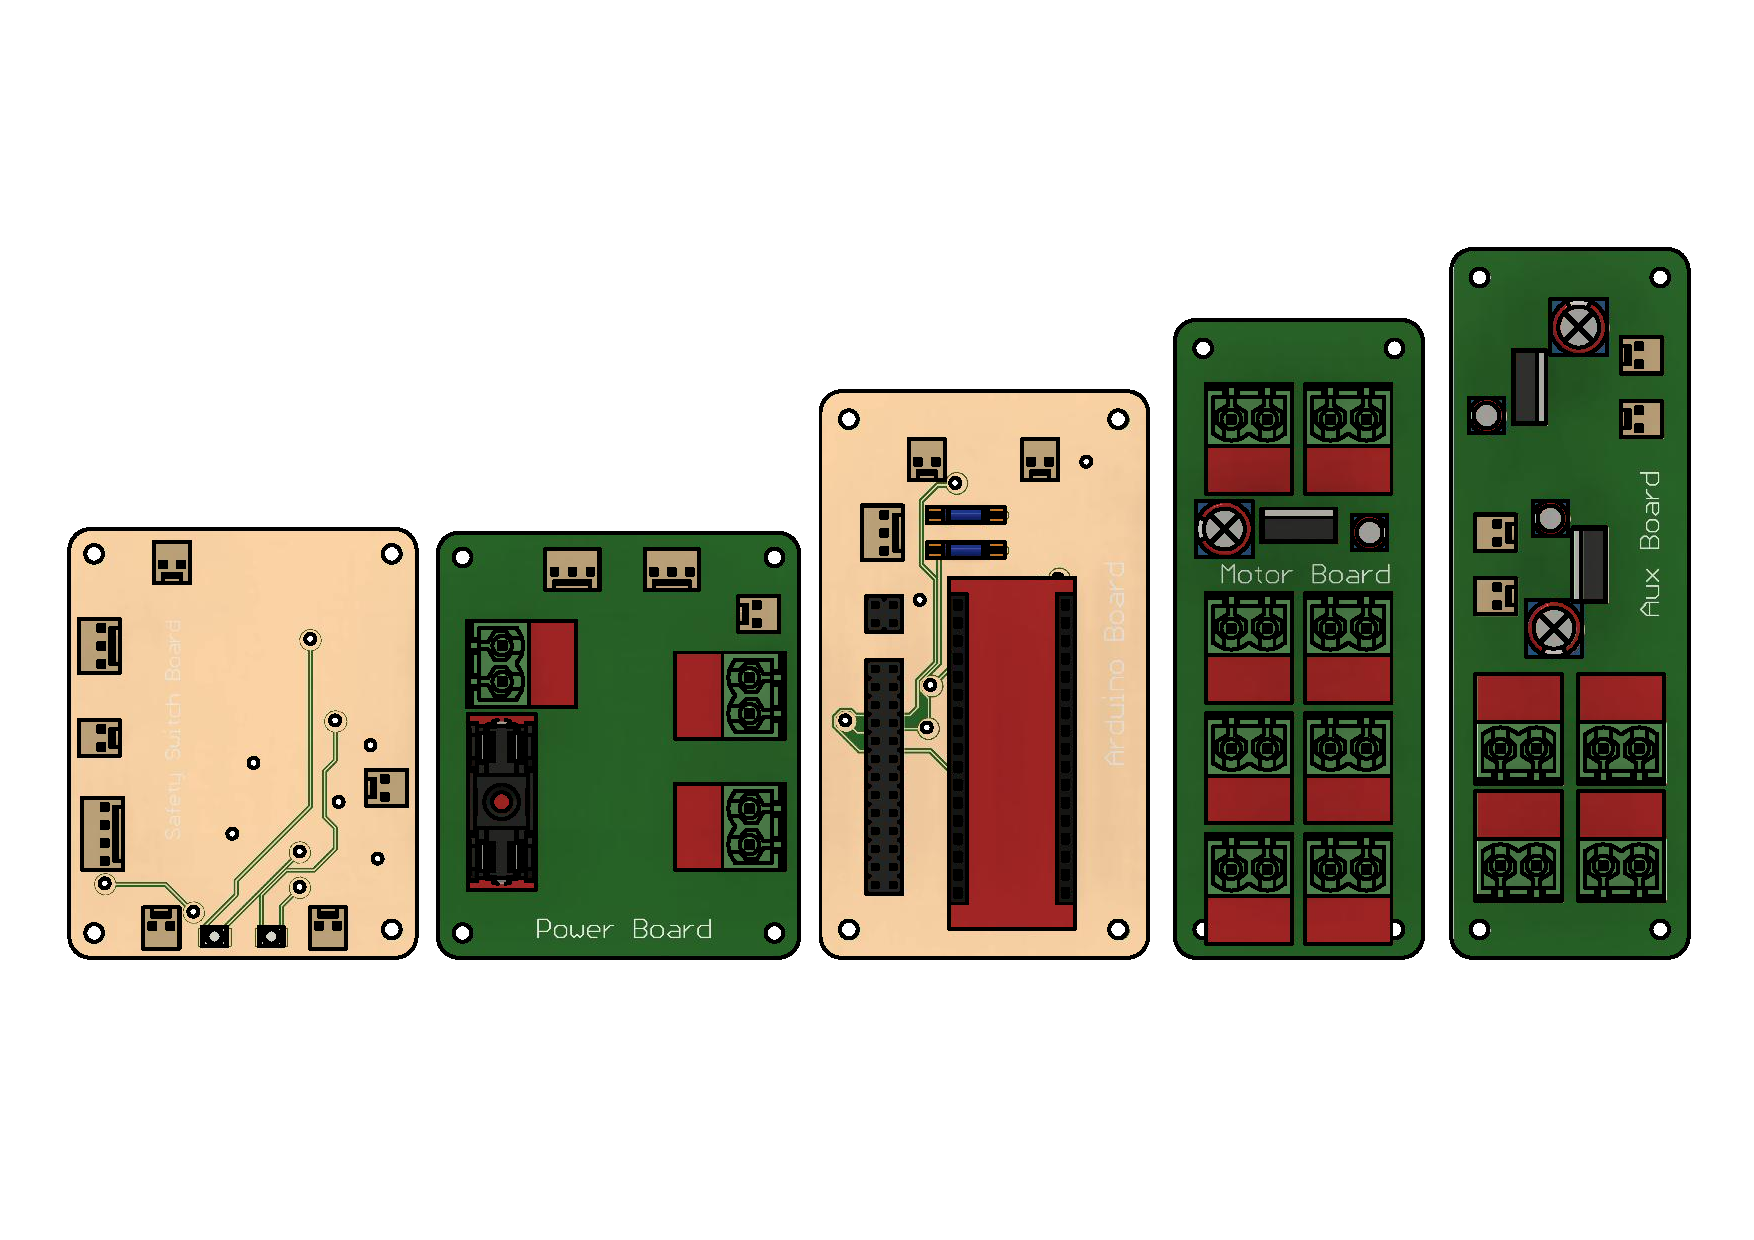
\includegraphics[width=1\textwidth]{Electronics/bulterpdb.pdf}
\caption{Top view of the boards in the PDB. From left to right: Safety Switch Board, Power Board, Arduino Board, Motor Board and Aux Board. The green areas are copper free areas and the red areas indicate connector clearance.}
\label{fig:butlerpdb}
\end{figure}

\subsubsection{Design}
The overall design to split the PDB into several boards has been chosen to simplify manufacturing and fault detection. This means that any issue is isolated to a single board and errors are more easily found. For complete specification of the boards see the manual. 

The Power Board is the main board that all power runs through. The power can be turned off with a main switch and the switching is done with MOSFETs\footnote{Metal–Oxide–Semiconductor Field-Effect Transistor}. The board has a fuse of 16 A installed to limit the maximum current. The Power Board has two power outputs controlled by the Safety Switch Board. The first output is the Motor output and it can supply a maximum of about 11 A. The second output is the auxiliary output and it can supply a maximum of about 10 A. 

The power is controlled from the Safety Switch Board. It controls the power to the outputs either from the main power switch or the safety switches. The board has four switches. The first switch is the main switch which controls the main power on or off. The second switch is a emergency switch which can disable the motors but having the control electronics enabled. The third switch is a magnetic switch that complements the emergency switch. A magnetic field need to be applied in the range of the magnetic switch to enable it. The fourth and last switch needs a "HIGH" digital signal in order to be enabled, this is controlled by the Arduino Board.
All switches are connected to an AND gate and needs to be "HIGH" for the Motor output to be enabled. In addition the Safety Switch Board as two LEDs, one green and one red, that indicate the status of the board. Green indicates that the board is on and all outputs are enabled and red indicates that at least one safety switch is not enabled so the motor output is disabled. Only one LED can be lit at the time.

The Motor Board is connected to the Power board and is basically an extension of the Power board. It has six outputs that use the battery voltage and two outputs that are regulated by a linear regulator at 12 V.

The Aux Board works by the same principle as the Motor board But is connected to the auxiliary output from the Power Board. It has four outputs that use the battery voltage and two 5 V and two 12 V linearly regulated outputs.

The Arduino board uses an Arduino Micro and communicates via I\textsuperscript{2}C bus connected to the Power Board were the voltage/current monitor is mounted. The Arduino Micro is programmed to monitor the voltage and current, this is to keep track of the voltage in order to determine when discharging of the battery should stop in order to protect the battery. The Arduino can then disable one of the safety switches which would disable the motors and the red LED will be lit. The Arduino board have been designed to be versatile with the pins from the Arduino Micro accessible for future functions.

\subsubsection{Future work}
The PDB have not been tested with the motors and the electronics, the only test that have been conducted is basic functionality. The PDB have not been wired on the Butler.

A battery have not been bought but the PDB was designed with the intention of using a LiFePO\textsubscript{4} battery from Biltema\footnote{\url{http://www.biltema.se/sv/}}. That battery have a voltage range of about 12.9 V to 14 V. If another battery with voltage below 12.9 V is going to be used, modifications need to be made to the PDB this is stated in the manual.

\subsection{System architecture - Ali Mokdad}
\begin{figure}[ht!]
\centering 
\includegraphics[width=1\textwidth]{Electronics/diagram.png}
\caption{Butler system architecture}
\label{fig:Butler system architecture}
\end{figure}

The system architecture of the Butler with the power requirements is shown in Figure~\ref{fig:Butler system architecture}. 
Table~\ref{table: The different motors for the Butler} lists brief explanation of each of the motors of the Butler.

\begin{table}[h!]
\centering
  \begin{tabular}{ | p{2cm}| p{9cm} |}
    \hline
    M1 arm  & Stepper motor for the first joint of the Butler arm   \\ \hline
    M2 arm  & Stepper motor for the second joint of the Butler arm   \\ \hline
    M3 arm  & Servo motor for rotating the hand. The feedback present in the diagram includes position, temperature, load, input voltage, etc.   \\ \hline
    M4 base & Dc motor with screw for moving all the arm up and down.\\ \hline
    M5 base & Stepper motor (same as M2 arm), for rotating the base of the Butler.\\
    \hline
  \end{tabular}
\caption{The different motors for the Butler}
\label{table: The different motors for the Butler}
\end{table}

\begin{table}[ht!]
\centering
  \begin{tabular}{ | p{2cm}| p{3cm} |}
    \hline
    M1 arm  & 14V, 0.4A    \\ \hline
    M2 arm  & 14V, 1.7A    \\ \hline
    M3 arm  & 12V, 2.2A    \\ \hline
    M4 base & 14V, 950 mA  \\ \hline
    M5 base & 14V, 1.7A    \\ \hline
    Cortex M4f & 5V        \\ \hline
    Jetson TX2 & 12 to 14V \\ \hline
  \end{tabular}
\caption{ Power requirements for the Butler}
\label{table: Power requirements for the Butler}
\end{table}

In the butler system: The PDB is responsible of providing power for the whole system. The Jetson TX2  is a full-featured development platform for visual computing, which constitutes the brain of the Butler; it communicates through a CAN bus with the Cortex M4f processor placed on a TM4C123G board which is an evaluation platform used for controlling the motors by sending the required PWM signals and serial communication (for the servo M3 hand) received from the Jetson TX2.
The LIDAR\cite{lidar} detection system which uses light from a laser to measure the distance to the object by illuminating that target with a pulsed laser light and send the data via USB communication to the Jetson TX2.
The Orbbec Astra Pro camera\cite{Camera} constitutes the eyes of the Butler, and the CHARLIE platform which is a different project platform will be used for this project. 